In this new chapter, we continue to drop some of the assumptions we've made so far and generalize the previously introduced model. One of the first assumption we made was that of restricting one item per machine. From now one however, not only one item can be produced by multiple machines but also one machine can produce multiple items. 

\section{Basis of the generalization}

Given that a machine $m$ can now produce more than one item, we introduce the production flow of item $i$ given by machine $m$, which we denote by $X(i,m)$, so that the overall production rate of item $i$ for the plant is given by \[ X(i) = \sum_m X(i,m) \]
What's more, we introduce the coefficient $\lambda(i,m), \forall i, \forall m$ which represents the contribution of machine $m$ in the overall production of item $i$. This contribution, expressed in percentage, is found as \[ \lambda(i,m) = \frac{X(i,m)}{X(i)} \] and it holds that $\sum_m \lambda(i,m) = 1$. 

As well, a direct generalization of what have been done previously gives the utilization of machine $m$ for producing item $i$ as \[ u(i,m) = \frac{X(i,m)}{\mu(i,m)} \] where $\mu(i,m)$ is a given data representing the maximum production rate of machine $m$ for item $i$. 

\begin{figure}[h!]
    \centering
    \begin{tikzpicture}
        \draw[->] (0,0) -- (10, 0);
        \draw (0,0) rectangle node {$"1"$} (2, .5);
        \draw (1, 1) node {$T_1$};

        \draw (3,0) rectangle node {$"3"$} (5, .5);
        \draw (4, 1) node {$T_2$};

        \draw (5, 0) rectangle node {$"1"$} (6, .5);
        \draw (5.5, 1) node {$T_3$};

        \draw (6.5, 0) rectangle node {$"2"$} (8, .5);
        \draw (7.25, 1) node {$T_4$};

        \draw (8, 0) rectangle node {$"3$} (9.5, .5);
        \draw (8.75, 1) node {$T_5$};

        \draw[decorate, decoration={brace, amplitude=5pt}] (10, -.2) -- (0, -.2);
        \draw (4.5, -.7) node[right] {$\sum T = \sum T_i + \textrm{idle time}$};

        \draw (13, 1) node {$u(1,m) = \dfrac{T_1 + T_3}{\sum T}$};
        \draw (13, 0) node {$u(2,m) = \dfrac{T_4}{\sum T}$};
        \draw (13, -1) node {$u(3,m) = \dfrac{T_2 + T_5}{\sum T}$};

    \end{tikzpicture}
    \caption{\label{shared_res:util}Machine utilisation with respect to a given item}
\end{figure}

From the example represented in figure (\ref{shared_res:util}), we can easily understand that $\sum_i u(i,m) \le 1$ (which basically means that a machine cannot be utilized more than its maximum production capacity). By substituting the newly introduced quantities in that inequality, and keeping in mind that $X(i) = X_fn_{if}$, it holds that
\[
    \begin{split}
        \sum_i u(i,m) \le 1, \forall m &\Leftrightarrow \sum_i\frac{X(i,m)}{\mu(i,m)} \le 1, \forall m\\
        \Leftrightarrow& \sum_i\frac{X(i)\lambda(i,m)}{\mu(i,m)} \le 1, \forall m\\
        \Leftrightarrow& \sum_i\frac{X_fn_{if}\lambda(i,m)}{\mu(i,m)} \le 1, \forall m\\
    \end{split}
\]
And since this set of inequality has to be fullfilled for every machine, then it holds that the only way to satisfy them all is to select $X_f$ as \begin{equation} X_f\le\min_m\left( \dfrac{1}{\sum_i\frac{n_{if}\lambda(i,m)}{\mu(i,m)}} \right) \label{shared_res:eqn_xfmax} \end{equation}

Note how, in the case of a single machine per item (i.e. $i=m$), it holds that $\lambda(i,m) = 1, \forall i=m$ and $0$ otherwise so that the minimum among all the machines becomes equivalent to the minimum among the items in such a way that the freshly established formula can be written as 
\[
    \min_m\left( \dfrac{1}{\sum_i\frac{n_{if}\lambda(i,m)}{\mu(i,m)}} \right) \overset{i=m}{=} \min_i\left( \dfrac{1}{ \frac{n_{if}}{\mu_i} } \right) = \min_i\left( \frac{\mu_i}{n_{if}} \right)
\] which is the formula we had found so far. 

\section{Model without setup time consideration}

If we do not consider the setup time of each machine, it still holds that $\mu(i,m) = \frac{1}{T_o(i,m)}$ which leads to the simplified following expression :
\begin{equation} X_f^{max}(\lambda) = \min_m\left( \frac{1}{ \sum_in_{if}\lambda(i,m)T_o(i,m) } \right) \label{shared_res:eqn_xf_wthout_setup} \end{equation} Thus, to determine the overall maximum production rate, one has to maximize, among all admissable values of $\underline\lambda$, the above expression. The problem can then be stated as follow : 
\[
    \begin{split}
        \underset{\underline\lambda}{\textrm{maximize }}& \min_m\left( \frac{1}{\sum_in_{if}\lambda(i,m)T_o(i,m)} \right)\\
        \textrm{subject to }& \sum_m \lambda(i,m) = 1, \forall i
    \end{split}
\]

\begin{wrapfigure}[10]{r}{4cm}
    \centering
    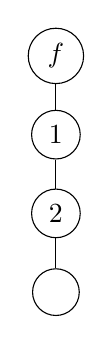
\begin{tikzpicture}[scale=.5]
        \draw (0,0) node[circle, draw] (f) {$f$};
        \draw (0,-2) node[circle, draw] (1) {$1$};
        \draw (0,-4) node[circle, draw] (2) {$2$};
        \draw (0,-6) node[circle, draw] (RM) {$\vphantom{f_i}$};

        \draw (RM) -- (2);
        \draw (2) -- (1);
        \draw (1) -- (f);
    \end{tikzpicture}
    \caption{\label{shared_res:bom1} Example}
\end{wrapfigure}

Let's consider the bill of material represented in figure (\ref{shared_res:bom1}) which depicts an assembly line. Two machines are present in the plant. The first machine, denoted $M_1$, can produce product $f$ and $1$ while the second one, $M_2$, can produce the products $1$ and $2$. The operational times of each machine for a given product are the following :
\begin{align*}
    T(f, M_1) &= 10 & T(1, M_1) &= 3 & T(2, M_2) &= 10 & T(1, M_2) &= 5
\end{align*}

Since some products can only be produced by specific machines, we can deduce some of the values of $\underline\lambda$. Indeed, it is clear that $\lambda(f,M_1) = 1$ and $\lambda(2, M_2) = 1$ and that $\lambda(f, M_2) = 0$ and $\lambda(2, M_1) = 0$. As regarding to the undetermined coefficients, we can at least, say that $\lambda(1, M_1) = 1 - \lambda(1, M_2)$ holds since product $1$ can be produced by both $M_1$ and $M_2$. Let's denote by $\lambda$ an arbitrary chosen coefficient among these two, let's say, $\lambda = \lambda(1, M_1)$. We can now compute the maximum production rate using equation (\ref{shared_res:eqn_xf_wthout_setup}) as follow :
\[
    X_f^{max}(\lambda) = \min\left( \frac{1}{1.10 + \lambda.3 + 0} ; \frac{1}{0+(1-\lambda).5+1.10} \right) = \min\left( \frac{1}{10+3\lambda} ; \frac{1}{15-5\lambda} \right)
\]
which is the function of $\lambda$ to be maximized. As it can  be seen in figure (\ref{shared_res:max_min_wthout_setup}), we have to maximize the function represented by a thick line which corresponds to the above computation. It is clear that the maximum is reached at the intercept of the two lines which is computed as \[ 3\lambda + 10 = 15 - 5\lambda\Leftrightarrow \lambda^\circ = \frac{5}{8} \] for which we find that \[ X_f^{max} = X_f^{max}(\lambda^\circ) = \frac{1}{3.\frac{5}{8}+10} = \frac{8}{95} \]

\begin{figure}[h!]
    \centering
    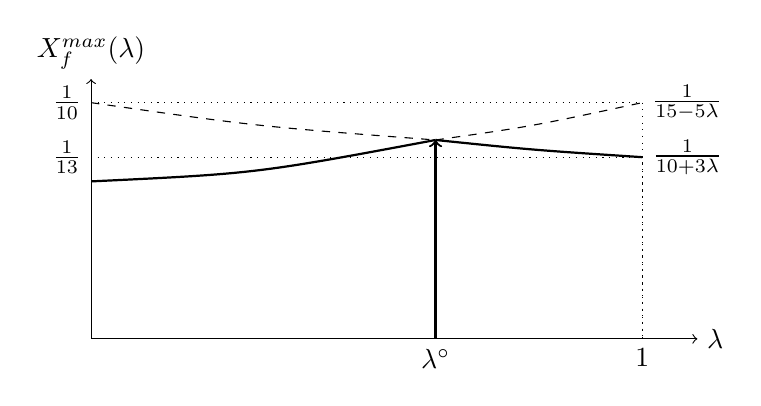
\begin{tikzpicture}[yscale=30, xscale=7]
        \draw[<->] (0, .11) node[above] {$X_f^{max}(\lambda)$} |- (1.1, 0) node[right] {$\lambda$};
        
        \draw[dotted] (0, .1) node[left] {$\frac{1}{10}$} -| (1, 0);
        \draw[dotted] (0, 1 / 13) node[left] {$\frac{1}{13}$} -| (1, 0) node[below] {$1$};

        \draw[thick] (0, 1/15) .. controls (.3, .07) .. (5/8, 8/95);
        \draw[dashed] (5/8, 8/95) .. controls (.8, .09) .. (1, .1) node[right] {$\frac{1}{15-5\lambda}$};

        \draw[thick] (5/8, 8/95) .. controls (.8, .08) .. (1, 1/13) node[right] {$\frac{1}{10+3\lambda}$};
        \draw[dashed] (0, .1) .. controls (.3, .09) .. (5/8, 8/95);

        \draw[->, thick] (5/8, 0) node[below] {$\lambda^\circ$} -- (5/8, 8/95);

    \end{tikzpicture}
    \caption{\label{shared_res:max_min_wthout_setup}Maximizing the minimum to find $X_f^{max}$}
\end{figure}

\section{Model with setup time (sequence independent)}

In this section, we add consideration for setup times with a simplifying assumption which is that setup times do not depend on the sequence of the items produced on one machine. This may not always be the case however. 

Similarly to what have been done when we firstly introduced the setup time in the second chapter, we can still consider the following to hold, with direct generalization : 
\begin{center}
    \begin{tikzpicture}
        \draw[->] (0, 0) node[left] {$m$} -- (5, 0);
        \draw[dotted] (.5, 0) rectangle (2, .5);
        \path (.5, .5) rectangle node {$T_{sm}$} (2, 1);
        \draw (2, 0) rectangle node {$b(i,m)$} (4.5, .5);

        \draw (8, .5) node {$\mu(i,m) = \dfrac{ b(i,m) }{ T_{sm} + b(i,m)T_o(i,m) }$};
    \end{tikzpicture}
\end{center}
Which yields from equation (\ref{shared_res:eqn_xfmax})
\[
    \begin{split}
        X_f^{max}(\underline\lambda, \underline b)
        &= \min_m\left( \frac{1}{ \sum_i\frac{ n_{if}\lambda(i,m)(T_{sm}+b(i,m)T_o(i,m)) }{b(i,m)} } \right)\\
        &= \min_m\left( \frac{1}{T_{sm}\sum_i\frac{n_{if}\lambda(i,m)}{b(i,m)} + \sum_i n_{if}\lambda(i,m)T_o(i,m)} \right)
    \end{split}
\] where $X_f^{max}$ is a function of $\underline\lambda$ and $\underline b$. We then have three possible cases :
\begin{itemize}
    \item Having fixed $\underline\lambda$, we can maximize $X_f^{max}$ with respect to $\underline b$. This bound is denoted by $\bar X_f^{max}(\underline\lambda) = \max_{\underline b}X_f^{max}(\underline\lambda, \underline b)$. Looking at the expression of $X_f^{max}$, one can notice that $\underline b$ appears only in one of the two term of the main sum, at the denominator. Thus, maximizing $X_f^{max}$ with respect to $\underline b$, having fixed $\underline\lambda$, can be done by assigning to $\underline b$ its maximum value $\underline b^{max}$.
    \item Having fixed $\underline b$, we can maximize $X_f^{max}$ with respect to $\underline \lambda$. This bound is denoted $\bbar X_f^{max}(\underline b) = \max_{\underline\lambda}X_f^{max}(\underline\lambda, \underline b)$
    \item Looking for the overall maximum production rate, we have to maximize $X_f^{max}$ with respect to both $\underline\lambda$ and $\underline b$. This bound is denoted $\bbbar X_f^{max} = \max_{\underline\lambda, \underline b}X_f^{max}$ which in fact, for the same reasons we have discussed for $\bar X_f^{max}$, can be computed as $\max_{\underline\lambda}\bar X_f^{max}(\underline\lambda)$
\end{itemize}

In order to use one of these bounds, i.e. choosing a smaller production rate $X_f^*$, one need to fullfill the constraints which derives from it. In that sense, let's suppose we want to use $X_f^*\le \bbbar X_f^{max}$. It holds that 
\[
    \begin{split}
        X_f^*\le \bbbar X_f^{max}
        &\Leftrightarrow X_f^{max}(\bbbar\lambda, \bbbar b) \ge X_f^*\\
        &\Leftrightarrow \frac{1}{ T_{sm}\sum_i\frac{n_{if}\lambda(i,m)}{b(i,m)} + \sum_i n_{if}\lambda(i,m)T_o(i,m) } \ge X_f^*, \forall m\\
        &\Leftrightarrow T_{sm}\sum_i n_{if}\frac{\lambda(i,m)}{b(i,m)} + \sum_i n_{if}\lambda(i,m)T_o(i,m) \le \frac{1}{X_f^*}, \forall m\\
        &\Leftrightarrow T_{sm}\sum_i n_{if}\frac{\lambda(i,m)}{b(i,m)} \le \frac{1}{X_f^*} - \sum_i n_{if}\lambda(i,m)T_o(i,m), \forall m
    \end{split}
\]

If this set of equations holds for given $X_f^*, \lambda$ and $b$ coefficients, then we can actually use $X_f^*$ as production rate for the plant with these value and the rate of each item is given by \[ X^*(i) = X_f^*n_{if} \] from which we can easily compute the production rate of each item per machine as \[ X^*(i,m) = X^*(i)\lambda(i,m) \] Having that in mind, how much time does machine $m$ needs to produce a batch of dimension $b(i,m)$ of product $i$ ? Simply enough, it is given by \[ D^*(i,m) = \frac{b(i,m)}{X_f^*n_{if}\lambda(i,m)} \] Similarly to what have been discussed in the early chapters, for it to be repeatable, the overall production cycle $D$ has to be a multiple of each particular machine production cycle $D^*(i,m)$. The minimum one being the \textit{least common multiple} of each $D^*(i,m)$ of the machines. Hence :
\[ D^* = \underset{i,m}{l.c.m}\textrm{ } D^*(i,m) \]

The next section will present an example of how to use these formulas.

\section{Multiple purpose machine : a first example}

Let's consider the bill of material depicted in figure (\ref{shared_res:bom2}) for which we have two different machines. Machine $M1$ can produce products $f, 1$ and $3$ while machine $M2$ can produce $2$ and $3$. We thus already know that $\lambda(1, M1) = \lambda(f, M1) = \lambda(2, M2) = 1$ and that $\lambda(1, M2) = \lambda(f, M2) = \lambda(2, M1) = 0$ since items $f, 1$ and $2$ can only be assigned to one single machine. The choice for $\lambda(3, M1)$ (and thus for $\lambda(3, M2)$) is left undetermined and we will denote it by $\lambda$ in the coming formulas. 

\begin{wrapfigure}[11]{l}{5cm}
    \centering
    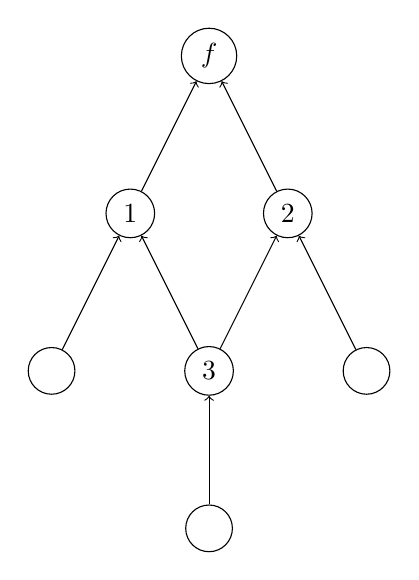
\begin{tikzpicture}[xscale=.5]
        \draw (0,0) node[circle, draw] (f) {$f$};
        \draw (-2,-2) node[circle, draw] (1) {$1$};
        \draw (2,-2) node[circle, draw] (2) {$2$};
        \draw (0,-4) node[circle, draw] (3) {$3$};
        \draw (-4,-4) node[circle, draw] (RM1) {$\vphantom{f_i}$};
        \draw (4,-4) node[circle, draw] (RM2) {$\vphantom{f_i}$};
        \draw (0,-6) node[circle, draw] (RM3) {$\vphantom{f_i}$};

        \draw[->] (RM3) -- (3);
        \draw[->] (RM1) -- (1);
        \draw[->] (RM2) -- (2);
        \draw[->] (3) -- (1);
        \draw[->] (3) -- (2);
        \draw[->] (1) -- (f);
        \draw[->] (2) -- (f);
    \end{tikzpicture}
    \caption{\label{shared_res:bom2}Bill of material}
\end{wrapfigure}

As well, the following operational times and setup times are given :
\begin{align*}
    T_o(f, M1) &= 8 &
    T_o(1, M1) &= 3 &
    T_o(3, M1) &= 2 &
    T_{sM1} &= 3\\
    T_o(2, M2) &= 6 &
    T_o(3, M2) &= 5 &
    &&
    T_{SM2} &= 0
\end{align*}

We are imposed to produce at a rate $X_f^* = \frac{1}{13}$. Let's first check if it is feasible to do so by computing the overall maximum production rate $\bbbar X_f^{max}$. As discussed earlier, $\bbbar X_f^{max}$ can be computed as $\max_{\underline\lambda}\bar X_f^{max}(\underline\lambda)$ where $\bar X_f^{max}$ is computed by inserted in formula (\ref{shared_res:eqn_xfmax}) the maximum batch sizes. In our case, there are no maximum batch size ($b^{max}_i = \infty$). This simplifies our problem in the following :
\[
    \begin{split}
        \bbbar X_f^{max} &= \max_{\underline\lambda, \underline b} X_f^{max}\\
        &= \max_{\underline\lambda, \underline b}\min_m\left( \frac{1}{ T_{sm}\sum_i\frac{n_{if}\lambda(i,m)}{b(i,m)} + \sum_i n_{if}\lambda(i,m)b(i,m) } \right)\\
        &\overset{b=\infty}{=} \max_{\underline\lambda}\min_m\left( \frac{1}{ \sum_i n_{if}\lambda(i,m)b(i,m) } \right) \\
        &= \max_{\underline\lambda} \min_m\left( \frac{1}{ 1.1.8 + 1.1.3 + 2.\lambda.2 } ; \frac{1}{ 1.1.6 + 2.(1-\lambda).5 } \right)\\
        &= \max_{\underline\lambda} \min_m\left( \frac{1}{ 11 + 4\lambda } ; \frac{1}{ 16 - 10\lambda } \right)
    \end{split} 
\]

Once again, the maximum value is reached when the two curves intercept, which is given by $11+4\lambda = 16-10\lambda$ which yields $\lambda^\circ = \frac{5}{14}$. For the sake of simplicity of computations, we will choose $\lambda = \frac{5}{15}=\frac{1}{3}$ which is close enough to the optimal one $\lambda^\circ$ but handier to manage. The value of $\bbbar X_f^{max}$ is then given by $\min_m\left( \frac{1}{ 11 + 4.\frac{1}{3} } ; \frac{1}{ 16 - 10\frac{1}{3} } \right) = \frac{3}{38}$. Note that $X_f^*\le \frac{3}{38}$. 

In order to choose the dimension of the bacthes, we need to fullfill the two following equations :
\[
    \begin{split}
        T_{sM1}\sum_i\frac{n_{if}\lambda(i,M1)}{b(i,M1)} \le \frac{1}{X_f^*} - \sum_in_{if}\lambda(i,M1)T_o(i,M1)\\
        T_{sM2}\sum_i\frac{n_{if}\lambda(i,M2)}{b(i,M2)} \le \frac{1}{X_f^*} - \sum_in_{if}\lambda(i,M2)T_o(i,M2)
    \end{split}
\]
Concerning machine $M2$ however, we know that $T_{sM2} = 0$ which gives \[ 0\le \frac{1}{X_f^*} - \sum_in_{if}\lambda(i,M2)T_o(i,M2) \] by re-writting the terms of this expression, one may realize that such a constraint is in fact always fullfilled when $X_f^*\le\bbbar X_f^{max}$ since, by definition (see (\ref{shared_res:eqn_xfmax})), \[ X_f^* \le \frac{1}{\sum_in_{if}\lambda(i,m)T_o(i,m)}, \forall m\textrm{ and }M2\textrm{ in particular} \]. 

Regarding machine $M1$ however, we have to find a triplet $(b(f,M1), b(1,M1), b(3,M1))$ which satisfies the first inequality, giving
\[
    \begin{split}
        3\left( \frac{1.1}{b(f,M1)} + \frac{1.1}{b(1,M1)} + \frac{2.\frac{1}{3}}{b(2,11)} \right) &\le 13 - \left( 11 + 4.\frac{1}{3} \right) \\
        \Leftrightarrow \frac{1}{b(f,M1)} + \frac{1}{b(1,M1)} + \frac{2}{3b(3,M1)} &\le \frac{2}{9}
    \end{split}
\]
Note that any triplet satisfying this latter equation yields a valid batch dimension. However, for the sake of simplicity, let's consider the case where $b(f,M1)=b(1,M1)=b(3,M1)=b$ which drives us to solve $\frac{1}{b} + \frac{1}{b} + \frac{2}{3b} \le \frac{2}{9}$ which is equivalent to $b\ge 12$. 

Let's choose to use $b(f,M1)=b(1,M1)=b(3,M1)=12$. What about $b(2,M2)$ and $b(3,M2)$ ? Since no constraints are imposed, we can randomly choose them while keeping feasibility of the solution. Let's choose $b(2,M2)=6$ and $b(3,M2)=12$. 

Let us now depict the production GANTT diagram by first computing the independent machine production cycles using $D(i,m) = \frac{b(i,m)}{X_f^*n_{if}\lambda(i,m)}$ : 
\begin{align*}
    D(f, M1) &= \frac{12}{\frac{1}{13}.1.1} = 12.13 &
    D(1, M1) &= \frac{12}{\frac{1}{13}.1.1} = 12.13 &
    D(3, M1) &= \frac{12}{\frac{1}{13}.2.\frac{1}{13}} = 3.6.13 \\
    D(2, M2) &= \frac{6}{\frac{1}{13}.1.1} = 6.13 &
    D(3, M2) &= \frac{12}{\frac{1}{13}.2.\frac{2}{3}} = 3^2.13
\end{align*}
The least common multiple gives us the overall production cycle $D$ as $D=2^2.3^2.13=468$. The associated GANTT diagram is represented in figure (\ref{shared_res:gantt1}).

\begin{figure}[h!]
    \centering
    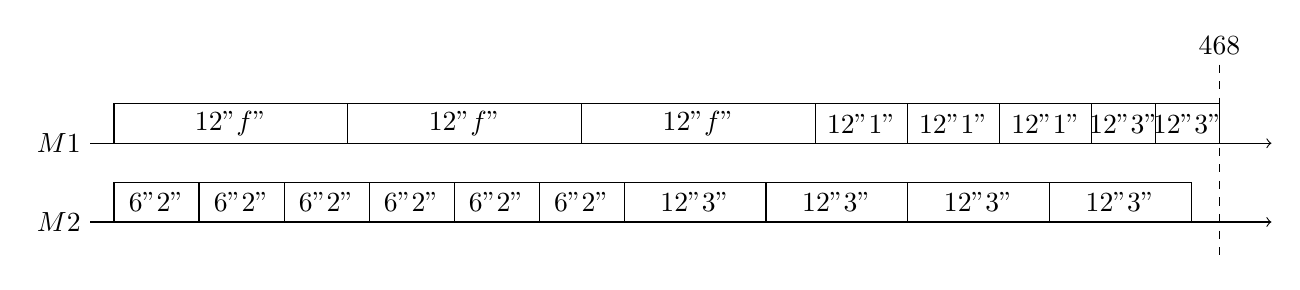
\begin{tikzpicture}[xscale=.03]
        \draw[->] (-10,0) node[left] {$M1$} -- (490, 0);

        % machine 1
        \foreach \k in {0,...,2} \draw (\k * 99, 0) rectangle node {$12"f"$} (\k * 99 + 99, .5);
        \foreach \k in {0,...,2} \draw (297 + \k * 39, 0) rectangle node {$12"1"$} (\k * 39 + 39 + 297, .5);
        \foreach \k in {0,...,1} \draw (414 + \k * 27, 0) rectangle node {$12"3"$} (\k * 27 + 27 + 414, .5);

        % machine 2
        \foreach \k in {0,...,5} \draw (\k * 36, -1) rectangle node {$6"2"$} (\k * 36 + 36, -.5);
        \foreach \k in {0,...,3} \draw (216 + \k * 60, -1) rectangle node {$12"3"$} (\k * 60 + 60 + 216, -.5);

        \draw[->] (-10,-1) node[left] {$M2$} -- (490, -1);

        \draw[dashed] (468, 1) node[above] {$468$} -- (468, -1.5);

    \end{tikzpicture}
    \caption{\label{shared_res:gantt1}GANTT diagram associated to the problem}
\end{figure}

\section{Practical computation}

The previous example has shown the relative complexity which arises with that formulation. In this new subsection, we will make a new assumption in order to simplify the computations. The assumption is relative to the bacth sizing and comes from the fact that by choosing $b(i,m) = \alpha(i,m)n_{if}\lambda(i,m)$ then the production cycle for each machine can be computed as \[ D(i,m) = \frac{\alpha(i,m)}{X_f} \] Thus, by choosing $\alpha(i,m)=\alpha,\forall i,m$ it holds that \[ D = \frac{\alpha}{X_f} \] (we avoid having to use the least common multiple of each $D(i,m)$ coefficients). 

From this assumption, we can re-write and simplify all the equations we have been considering so far. Let's start with the expression of $X_f^{max}$ as introduced in equation (\ref{shared_res:eqn_xfmax}). However, one must pay attention to the fact that we can NOT directly substitute $b(i,m)$ by $\alpha n_{if}\lambda(i,m)$ since writting $T_{sm}\sum_i\frac{n_{if}\lambda(i,m)}{\alpha n_{if}\lambda(i,m)}$ would imply a division by $0$ in the case where $\lambda(i,m) = 0$. But rather, we should use the following : 
\[
    T_{sm}\sum_{\underset{\lambda(i,m)\ne 0}{i}} \frac{n_{if}\lambda(i,m)}{\alpha n_{if}\lambda(i,m)}
    = T_{sm}\sum_{\underset{\lambda(i,m)\ne 0}{i}} \frac{1}{\alpha}
\]
which, by introducing $\gamma(m) = \sum_{\underset{\lambda(i,m)\ne 0}{i}} 1$ (which represents the number of different items machine $m$ will actually produce), can be better written as
\[
    \frac{T_{sm}}{\alpha}\gamma(m)
\]
Hence the final formula expressing $X_f^{max}$ as 
\[
    X_f^{max} = \min_m\left( \frac{1}{ \frac{T_{sm}}{\alpha}\gamma(m) + \sum_i n_{if}\lambda(i,m)T_o(i,m) } \right)
\]

That being said, one should keep in mind that in the most general case, one has to respect the constraint stipulating that $b^{min}(i,m)\le b(i,m) \le b^{max}(i,m),  \forall i,m$ for when $m$ produces $i$ (otherwise the batch size is off course $0$). This yields to the following development :
\[
    \begin{split}
        b^{min}(i,m) \le \alpha n_{if}\lambda(i,m) \le b^{max}(i,m)
        &\Leftrightarrow
        \frac{ b^{min}(i,m) }{ n_{if}\lambda(i,m) } \le \alpha \le \frac{ b^{max}(i,m) }{ n_{if}\lambda(i,m) }, \forall m,i\\
        &\Leftrightarrow
        \max_{i,m}\left( \frac{ b^{min}(i,m) }{ n_{if}\lambda(i,m) } \right) \le \alpha \le \min_{i,m}\left( \frac{ b^{max}(i,m) }{ n_{if}\lambda(i,m) } \right)
    \end{split}
\]
so that $\alpha$ should be chosen among this interval while giving every $b(i,m)$ an integer value. If such a choice is not possible, then one cannot use this simplification and has to deal with the original problem statement. 

Concerning $\bar X_f^{max}$ it now simply becomes $X_f^{max}(\alpha^{max}, \lambda)$ in such a way that if $\alpha^{max}=\infty$ then
\[
    \bar X_f^{max} = \min_m\left( \frac{1}{\sum_i n_{if}\lambda(i,m)T_o(i,m)} \right)
\]
while if $\alpha^{max}<\infty$ then it holds that
\[
    \bar X_f^{max} = \min_m\left( \frac{1}{ \frac{T_{sm}\gamma(m)}{\alpha^{max}} + \sum_i n_{if}\lambda(i,m)T_o(i,m)} \right)
\]

One may argue however that, when computing the maximum of $X_f^{max}$ with respect to any of its arguments, we may not know the value of $\gamma(m)$. This is true and the choice for the value $\gamma(m)$ has to be done \textit{a priori}. Of course, $\gamma(m)$ has to be at least equal to the number of items it is the only machine to produce. As well, the following situation may happen : let's fix for a given machine $m$ the number of different items it will actually produce to $4$, $\gamma(m) = 4$. Solving for $\underline \lambda$ may lead to a solution in which only three different $\lambda(i,m)$ are non zero valuated (which violates the fact that $\gamma(m) = 4$). Dually, by fixing $\gamma(m) = 3$ on the same instance, the solution for $\underline \lambda$ may yield four $\lambda(i,m)$ coefficients different from zero. This is due to the fact that $\gamma(m) = f(\underline \lambda)$ and that we should regard this problem as a global optimization problem. 

\section{Production time}

Using the assumption according to which $b(i,m) = \alpha n_{if}\lambda(i,m)$, we can write the following relation : $b(f,m) = \alpha\lambda(f,m)$ which, by summing over the different machines gives : 
\[ \sum_mb(f,m) = \alpha\sum_m\lambda(f,m)=\alpha \]
which means that, during one production cycle, exactly $\alpha$ final products are produced by the plant. What is the time needed to produce the first $\alpha$ final items ? Again, we can approximate it by $L\times D$ where $D$ is the production cycle and $L$ the number of level of the bill of material (the longest length from the leaves to the root). Thus, let's say we want to estimte the time needed to produce the $N$ final items. We first need to produce the first $\alpha$ final items starting from scracth then produce $\left\lceil\frac{N}{\alpha}\right\rceil - 1$ other final items. Thus the generalized formula :
\[
    T_{prod}(N)|_\alpha = \left(L-1 + \left\lceil \frac{N}{\alpha} \right\rceil \right).D
\] where $D = \frac{\alpha}{X_f}$

What's more, and much similarly to what we have been doing so far, by assuming that machine $b$ is the bottleneck machine, we can write that 
\[
    D = \dfrac{ \alpha }{
        \frac{1}{
            \frac{T_{sb}\gamma(b)}{\alpha}
            + \sum_i n_{if}\lambda(i,b)T_o(i,b)
        }
    } = T_{sb}\gamma(b) + \alpha\sum_i n_{if}\lambda(i,b)T_o(i,b)
\] in such a way that 
\[
    T_{prod}(N)|_\alpha = \left(L-1 + \left\lceil \frac{N}{\alpha} \right\rceil \right)\left( T_{sb}\gamma(b) + \alpha\sum_i n_{if}\lambda(i,b)T_o(i,b) \right)
\]

The latter result can be regarded as a function of $\alpha$ which we can derive and solve for the optimal. Doing so yields the following :
\[
    \nabla. = 0 \Leftrightarrow \alpha^\circ =
    \sqrt{
        \dfrac{
            NT_{sb}\gamma(b)
        }{
            (L-1)\sum_i n_{if}\lambda(i,b)T_o(i,b)
        }
    }
\]Pay attention to the fact that this result holds if, and only if, the \textit{a priori} chosen bottleneck machine is well \textit{a posteriori} the bottleneck machine corresponding to the $\alpha$ value which has been found. 

\section{One final example}

This section will now present the final example of this chapter. 
